In this chapter we present and discuss the results of our empirical performance study of the Fribourg construction. The presentation of the results is structured along the two sub-studies of the internal tests and the external tests.

Section~\ref{5_internal} presents the results of the internal tests, and Section~\ref{5_external} presents the results of the external tests. Both sections have two subsections. The first one for the results of the \goal{} test set, and the second one for the results of the Michel test set.

In Section~\ref{5_discussion} we summarise and discuss the most important results and insights gained from the study. Finally, in Section~\ref{5_limitations}, we identify the limitations of our study.


\section{Internal Tests}
\label{5_internal}
For the internal tests we tested different versions of the Fribourg construction with both, the \goal{} test set and the Michel test set.

For the \goal{} test set, the tested versions are (see Section~\ref{4_internal}):
\begin{enumerate}
\item Fribourg
\item Fribourg+R2C
\item Fribourg+R2C+C
\item Fribourg+M1
\item Fribourg+M1+M2
\item Fribourg+M1+R2C
\item Fribourg+M1+R2C+C
\item Fribourg+R
\end{enumerate}

For the Michel test set, the tested versions are (again, see Section~\ref{4_internal}):
\begin{enumerate}
\item Fribourg
\item Fribourg+R2C
\item Fribourg+M1
\item Fribourg+M1+M2
\item Fribourg+M1+M2+R2C
\item Fribourg+R
\end{enumerate}

Below, we present the results for the \goal{} and the Michel test set in separate sections.

\subsection{GOAL Test Set}
\label{5_internal_goal}

\subsubsection{Overall}
Before analysing the actual results, let us see how many aborted complementations tasks there are, so that we can determine the effective samples, which is the set of results that we will actually analyse. Table~\ref{i.g.out_table} shows the number of timeouts and memory excesses for each of the eight tested versions of the Fribourg construction.

\begin{table}[ht]
\centering
% latex table generated in R 3.1.2 by xtable 1.7-4 package
% Sat Jun  6 16:42:17 2015
\begin{tabular}{lrr}
  \hline
Construction & Timeouts & Memory excesses \\ 
  \hline
Fribourg & 48 & 0 \\ 
  Fribourg+R2C & 30 & 0 \\ 
  Fribourg+R2C+C & 54 & 0 \\ 
  Fribourg+M1 & 2 & 0 \\ 
  Fribourg+M1+M2 & 1 & 0 \\ 
  Fribourg+M1+R2C & 1 & 0 \\ 
  Fribourg+M1+R2C+C & 8 & 0 \\ 
  Fribourg+R & 48 & 0 \\ 
   \hline
\end{tabular}

\caption{Number of timeouts and memory excesses in the internal tests with the \goal{} test set.}
\label{i.g.out_table}
\end{table}

As we can see in Table~\ref{i.g.out_table}, there are no memory excesses at all. That is, none of the 11,000 complementation tasks needed more than 1 GB Java heap memory. However, there is quite a number of timeouts. The versions Fribourg, Fribourg+R2C, Fribourg+R2C+C, and Fribourg+R all have 30 or more timeouts. All the other versions, which are the ones containing the M1 optimisation, have only 8 or less timeouts.

If we determine the effective samples from these results, we get a number of 10,939 automata. That is, 61 automata (0.55\%) are excluded from the effective samples, because their complementation has been aborted for at least one of the versions.

The entire remaining result analysis in this section will be based on these 10,939 effective samples. Our main interest are the sizes of the complements of these 10,939 automata. To get a first impression, we plot all these complement sizes as a stripchart in Figure~\ref{i.g.stripchart}. Each strip contains a dot for each of the 10,939 automata that indicates its complement size. Thus, each strip in Figure~\ref{i.g.stripchart} contains exactly 10,939 dots.

\begin{figure}[ht]
\centering
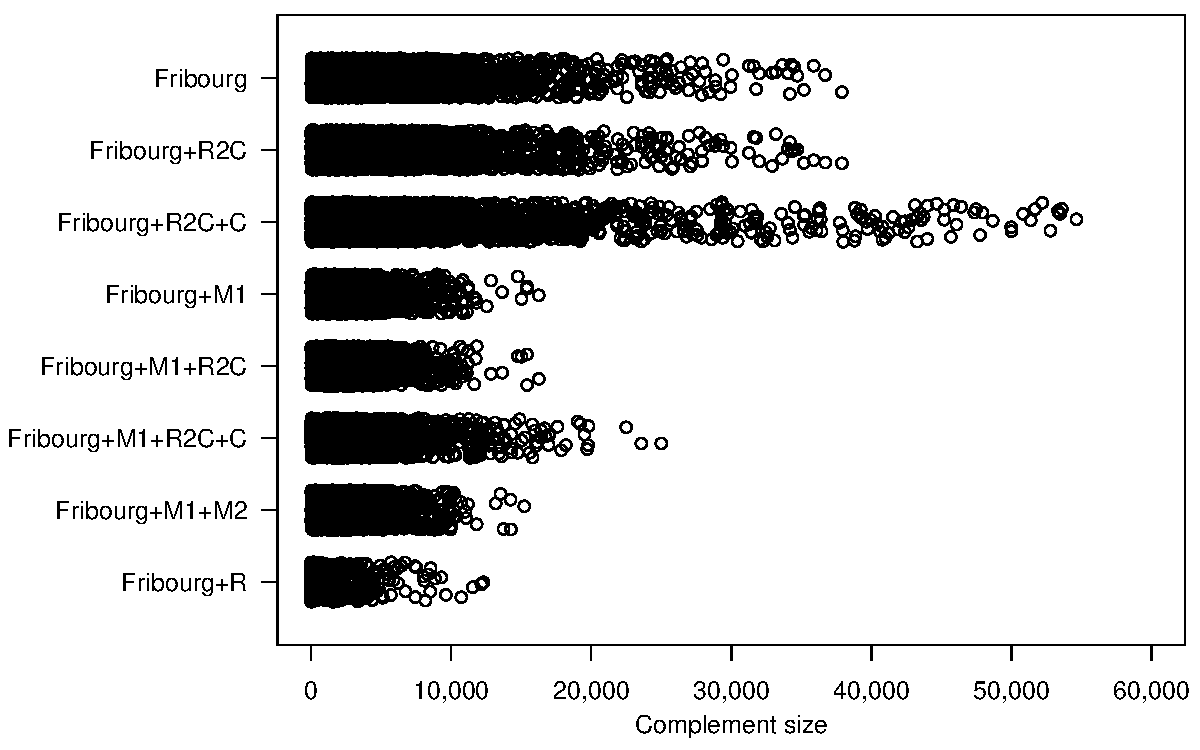
\includegraphics[width=0.7\textwidth]{figures/r/internal/goal/s.stripchart.pdf}
\caption{Stripchart with the complement sizes of the 10,939 effective samples of the \goal{} test set.}
\label{i.g.stripchart}
\end{figure}

One thing to note is that the distribution of complement sizes is right-skewed (also known as positive-skewed). That means, there is a long tail towards the right along the $x$-axis. The peak seems to be close to the left end of the $x$-axis. This means that most of the complements are small and there are fewer and fewer complements with bigger sizes. A right-skewed distribution implies that the mean is generally higher than the median. This is because the mean is ``dragged'' to the right by the few large values.

The most interesting thing in Figure~\ref{i.g.stripchart} is however to compare the distributions of the different versions with each other, especially the tail sizes. Going from top to bottom, the distributions of Fribourg and Fribourg+R2C have similarly long tails. Fribourg+R2C+C, however, has a considerably longer tail. This shows us that the C option has a significant effect on the complement sizes, because it adds an additional state to the automata which are not complete. As we have seen in Section~\ref{4_goal_testset}, only 9\% of the automata of the \goal{} test set are complete, thus 91\% of the automata are enlarged in this way. This might be the cause for the bigger number of larger complements.

Next, Fribourg+M1, Fribourg+M1+M2, and Fribourg+M1+R2C all have similarly long tails. However, these tails are significantly shorter than the ones of the previous three versions. This indicates that the M1 optimisation is very effective in reducing the complement sizes. The distribution of Fribourg+M1+R2C+C again has a longer tail than the corresponding version without the C option, as we just discussed above.

Finally, the distribution of Fribourg+R has a very short tail. The Fribourg+R version is a special case, because it is essentially the Fribourg version where all the unreachable and dead states are removed from the produced complements. Thus, if we compare the results of Fribourg and Fribourg+R, then we get an idea of how man unreachable and dead states are produced by the Fribourg version.

The stripchart in Figure~\ref{i.g.stripchart} gave us a first impression about the resulting complement sizes. However, for further analysis, we need statistics. In Table~\ref{i.g.stats_table} we show such statistics about the complement sizes. They consist of the mean together with the classic five-number summary, consisting of minimum value, 25th percentile, median, 75th percentile and maximum value.

\begin{table}[ht]
\centering
% latex table generated in R 3.1.2 by xtable 1.7-4 package
% Sat Jun  6 16:42:20 2015
\begin{tabular}{lrrrrrr}
  \hline
Construction & Mean & Min. & P25 & Median & P75 & Max. \\ 
  \hline
Piterman+EQ+RO & 209.6 & 1 & 38.0 & 80.0 & 183.0 & 20,349 \\ 
  Slice+P+RO+MADJ+EG & 949.4 & 2 & 120.0 & 396.0 & 1,003.0 & 41,081 \\ 
  Fribourg+M1+R2C & 1,017.3 & 2 & 153.0 & 452.0 & 1,134.0 & 37,068 \\ 
   \hline
\end{tabular}

\caption{Statistics of the complement sizes of the 10,939 effective samples of the \goal{} test set.}
\label{i.g.stats_table}
\end{table}

As we can see, the mean is indeed throughout higher than the median, which is typical for right-skewed distributions. Regarding the characteristics of the median and the mean, the median is generally the more ``robust'' statistics, because it is not affected by the actual values of the data points at both sides of the median point. The mean, on the other hand, is a function of all the values in the distribution and thus may be affected by, for example, extraordinarily high values of outliers (as in our case). For our analysis, we will therefore mostly use the median. However, we will sometimes refer to the mean too, as well as for the other statistics in Table~\ref{i.g.stats_table}.

If we go through the median values in Table~\ref{i.g.stats_table} we encounter some surprises. To begin with, as expected, there is a decrease from Fribourg (761) to Fribourg+R2C (689). Then, however, there is a significant drop to 451 with Fribourg+R2C+C. This is a surprise insofar as by looking at Figure~\ref{i.g.stripchart}, Fribourg+R2C+C seems to have the worst performance at a first glance. Indeed it also has the highest mean, which is due to the group of extremely large complements. The median, however, is very low, even lower than the one of Fribourg+M1 with its significantly shorter tail in Figure~\ref{i.g.stripchart}. Also the 25th percentile of Fribourg+R2C+C is with 85 one of the lowest. Going to the other side of the median, however, the 75th percentile (2,329) is the largest of all versions. A possible characterisation of this phenomenon is that the C option (together with R2C) makes small complements smaller, and large complements larger. The diminishment of small complements is far-reaching enough that the median is affected by it and decreased significantly.

The next thing we see in Table~\ref{i.g.stats_table} is that the median of Fribourg+M1 (482) is slightly lower than the median of Fribourg+M1+M2 (496). The same applies to the 25th and 75th percentile. This means that the additional application of the M2 optimisation to Fribourg+M1 \textit{decreases} the performance of the construction on the \goal{} test set. The difference is rather small (the median increase from Fribourg+M1 to Fribourg+M1+M2 is 2.9\%). However, it is still enough for us to consider Fribourg+M1 as the more performant of the two versions.

Fribourg+M1+R2C brings down the median from 482 to 447, with respect to Fribourg+M1. Also the 25th and 75th percentile are decreased. Adding the C option to Fribourg+M1+R2C, again causes the median to drop dramatically, from 447 to 331. The 25th percentile decreases from 152 to 83. The 75th percentile however increases from 1,118 to 1,208.5. Here we have again the same picture of the effect of adding the C option that we had before. Namely that small complements are made smaller, and large complements are made larger.

Finally, the last row in Table~\ref{i.g.stats_table} with Fribourg+R shows the extent of unreachable and dead states that the Fribourg version produces. The median is 1, and a further analysis reveals that also the 61st percentile is 1. Only from the 62nd percentile onwards the complement sizes start to increase. This means that 61\% of the complements have a size of 1, if we remove all the unreachable and dead states This is not so surprising, because we know from Section~\ref{4_goal_testset} that 61.8\% of the automata in the \goal{} test set are universal, which means that their complements may contain only a single state.

\subsubsection{Per-Class}
Up to now, we only looked at statistics that are aggregated over the entire test set. This mixes together all the automata of the 110 transition density/acceptance density classes of the \goal{} test set with their very different characteristics (see the description of the \goal{} test set in Section~\ref{4_goal_testset}). However, it would be interesting know more about the complement sizes of specific classes, so that we can for example identify easy and hard automata. Therefore, in this part of the analysis, we look at statistics on a per-class basis. This means that for each construction version we will have not just one value per statistics (for example, one median), but 110 values, namely one for each class (for example, 110 medians). Given this complexity, we will restrict ourselves to the median statistics, which we already identified as the most significant and robust statistics. Thus, in the following, we will analyse the median complement sizes of the 110 classes of the \goal{} test set.

These per-class statistics result in a similar type of per-class data that we had when we analysed the number of complete, universal, and empty automata in the 110 classes of the \goal{} test set in Section~\ref{4_goal_testset}. There, we presented this data in two forms, as matrices and as perspective plots. The advantage of matrices is that they show all values unambiguously, the advantage of perspective plots is that they show the relative differences between classes and the overall pattern more intuitively. In this chapter we will only use perspective plots to present this data. This is mainly for space reasons. However, we present the corresponding matrices of all the perspective plots of this chapter in Appendix~\ref{app_matrices}.

Figures~\ref{i.g.persp_1} and~\ref{i.g.persp_2} show the perspective plots for the eight tested Fribourg construction versions. The spatial orientation of these perspective plots corresponds to looking at a matrix from the lower-right corner. That is, the corner of the perspective plots that is closest to the viewer corresponds to the lower-right corner of the corresponding $11 \times 10$ matrices. This orientation will be the same for all the remaining perspective plots in this thesis. The surface colours of the perspective plots are in function of the vertical ``height'' of the surface. They are chosen to draw an analogy with physical terrain. In this sense, we will often talk of ``mountains'', ``hills'', and ``flatland'' in the perspective plots.

\newcommand{\perspwidth}{0.475}

\begin{figure}[ht]
\centering
  \hfill
  \begin{subfigure}[t]{\perspwidth\textwidth}
  \centering
  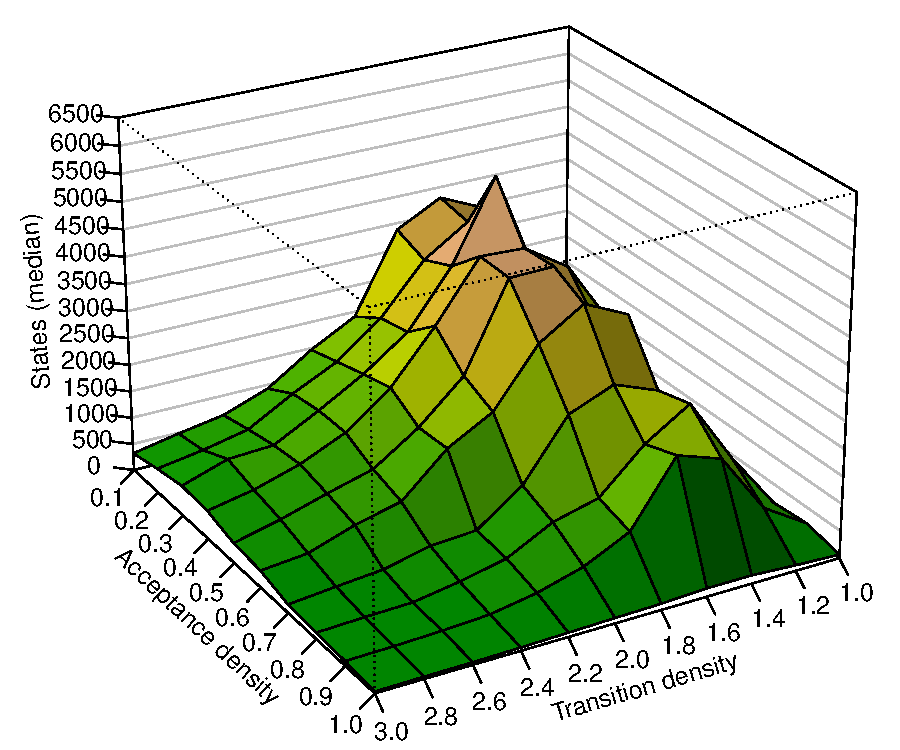
\includegraphics[width=\textwidth]{figures/r/internal/goal/s.median.Fribourg.pdf}
  \caption{Fribourg}
  \end{subfigure}
  \hfill
  \begin{subfigure}[t]{\perspwidth\textwidth}
  \centering
  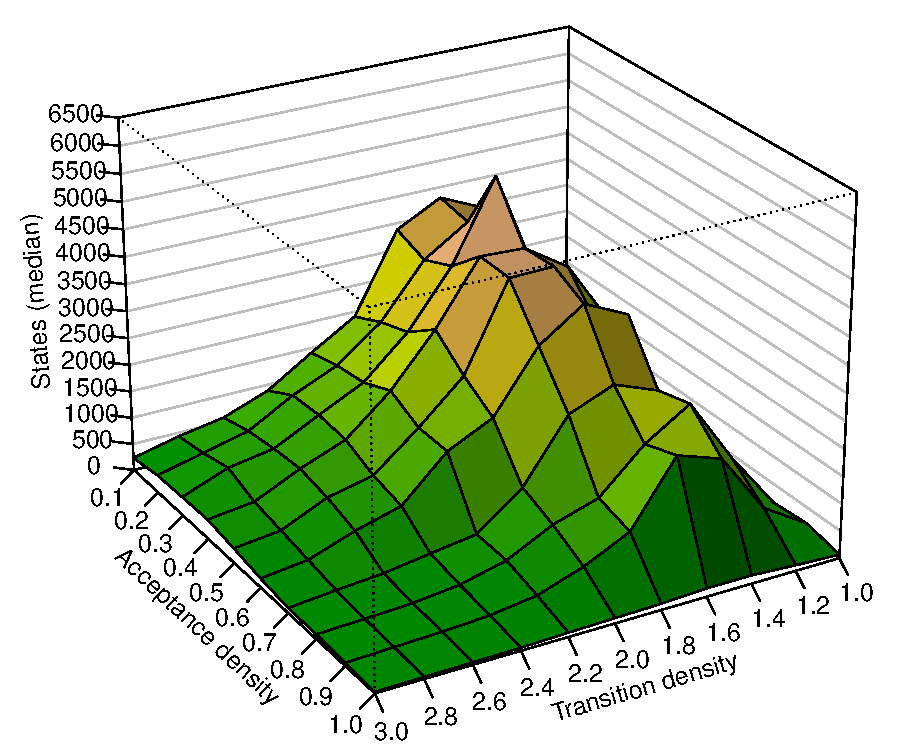
\includegraphics[width=\textwidth]{figures/r/internal/goal/s.median.Fribourg+R2C.pdf}
  \caption{Fribourg+R2C}
  \end{subfigure}
  \hfill

  \hfill
  \begin{subfigure}[t]{\perspwidth\textwidth}
  \centering
  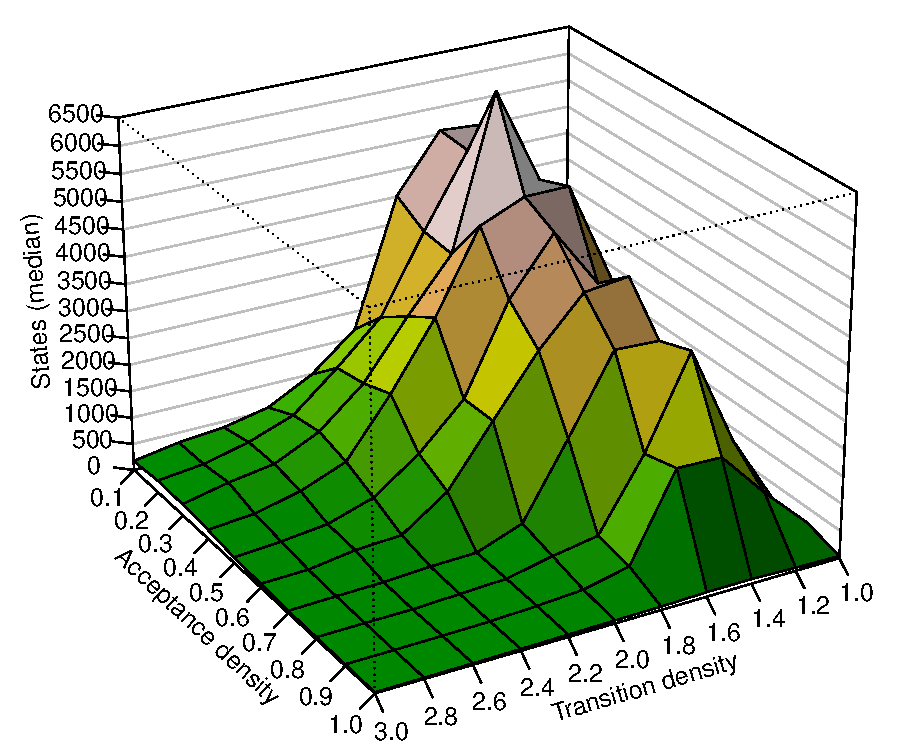
\includegraphics[width=\textwidth]{figures/r/internal/goal/s.median.Fribourg+R2C+C.pdf}
  \caption{Fribourg+R2C+C}
  \end{subfigure}
  \hfill
  \begin{subfigure}[t]{\perspwidth\textwidth}
  \centering
  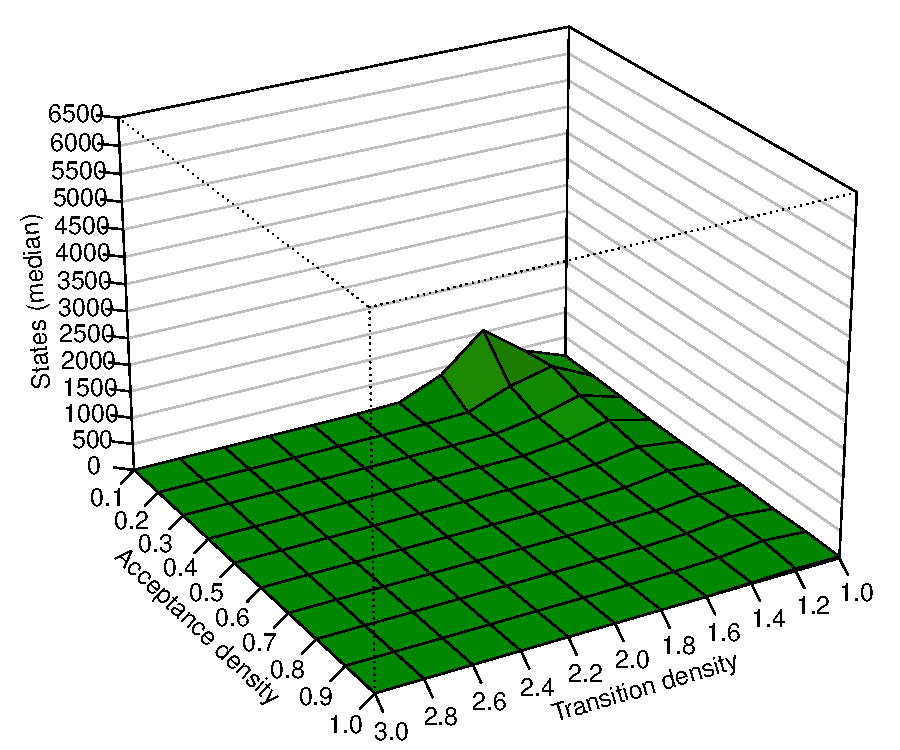
\includegraphics[width=\textwidth]{figures/r/internal/goal/s.median.Fribourg+R.pdf}
  \caption{Fribourg+R}
  \end{subfigure}
  \hfill  
\caption{Median complement sizes of the 10,939 effective samples from the \goal{} test set for each of the 110 classes.}
\label{i.g.persp_1}
\end{figure}

The most apparent information that the perspective plots convey is that there are indeed large differences in the complement sizes across the 110 classes. In all the construction versions there is a mountain, or at least a hill, very roughly in the area between transition densities of 1.2 and 2.4, and acceptance densities of 0.1 and 0.9. The mountain is oblong, and its ridge runs across the entire spectrum of the acceptance densities. The top of the ridge is roughly at a transition density of 1.6. On the higher end of the acceptance density spectrum (acceptance density 1.0) the mountain is flattened to a height close to zero. On the other end of the acceptance density spectrum (acceptance density 0.1), however, the mountain stays high.

Considering these median complement sizes in the perspective plots, apparently the automata of, for example, the class with a transition density of 1.6 and an acceptance density of 0.3 result in much larger complements than the automata of, for example, the class with a transition density of 3.0 and an acceptance density of 1.0. We could say that the automata of the first class are harder than the automata of the second class. Later in this section, we will try to identify hard, medium, and easy classes. For now, we will however focus on the relative differences between the different versions of the Fribourg construction.

Looking at the perspective plots in Figure~\ref{i.g.persp_1}, the plots for Fribourg and Fribourg+R2C are rather similar. The top of the mountain ridge is between 3,500 and 4,000 states with a single peak of around 4900 states in the class with transition density 1.6 and acceptance density 0.3. From Table~\ref{i.g.stats_table} we can learn that the overall median complement size is 761 for Fribourg and 689 for Fribourg+R2C. These low values might surprise at first as the mountain, which is much higher, seems to dominate. However, by taking a closer look, it becomes apparent that around half of the classes are in rather low terrain (less than 1,000 states). Furthermore, the heights of the mountain peak do not allow to deduce anything about the overall median, because the median is not affected by the actual values of the data points which are greater than the median. The overall mean complement sizes of Fribourg and Fribourg+R2C in turn are 2,004.6 and 1955.9, respectively. 

Fribourg+R2C+C in Figure~\ref{i.g.persp_1} (c) has an even higher mountain than the Fribourg and Fribourg+R2C. The top of the ridge is at around 5,000 states and the peak at the class 1.6/3.0 has close to 6,500 states. As already in the stripchart in Figure~\ref{i.g.stripchart}, Fribourg+R2C+C seems much worse than Fribourg+R2C at a first glance. However, as we have seen in Table~\ref{i.g.stats_table}, the median of Fribourg+R2C+C is 34.5\% lower than the median of Fribourg+R2C (689 to 451). By taking a closer look at the perspective plots of Fribourg+R2C and Fribourg+R2C+C, the reason for this can be seen. The low areas of Fribourg+R2C+C are slightly lower than the low areas of Fribourg+R2C. This is apparently enough to decrease the overall median. The much higher mountain peaks of Fribourg+R2C+C, on the other hand, do not influence the median. However, they show their effect in the overall mean which for Fribourg+R2C+C is 24\% higher than for Fribourg+R2C (2,424.6 to 1,955.9).

Comparing the fourth plot in Figure~\ref{i.g.persp_1}, Fribourg+R, to the plots of Fribourg, Fribourg+R2C, and Fribourg+R2C+C is like comparing a Dutch polder to the Swiss Alps. The mountain shrinks to a small hillock and the rest of the terrain is low and flat. This is because so many complements of the Fribourg construction can be reduced to very small sizes by removing their unreachable and dead states. The corresponding matrix in Appendix~\ref{app_matrices} reveals that 68 of the 110 classes have a median complement size of 1. If we further compare this matrix to the matrix with the number of universal automata in Figure~\ref{testset_analysis} (b) in Section~\ref{4_goal_testset}, we see that all the classes with a median of 1 contain more than 50 universal automata, and the classes with a median greater than 1 contain less than 50 universal automata. There is a total of 100 automata per class. This makes sense as the complements of universal automata are empty automata, and every empty automaton can be reduced to an automaton with a single non-accepting state. Looking at the classes with a median greater than 1, we see that their values are still considerably lower than the ones of the plain Fribourg construction.

\begin{figure}[ht]
\centering
  \hfill
  \begin{subfigure}[t]{\perspwidth\textwidth}
  \centering
  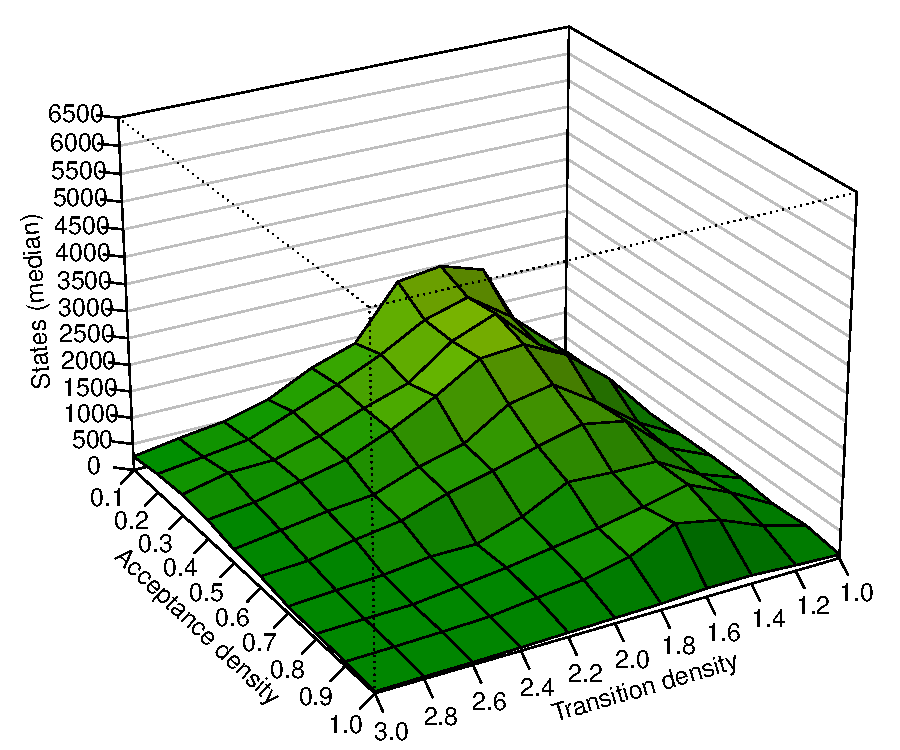
\includegraphics[width=\textwidth]{figures/r/internal/goal/s.median.Fribourg+M1.pdf}
  \caption{Fribourg+M1}
  \end{subfigure}
  \hfill
  \begin{subfigure}[t]{\perspwidth\textwidth}
  \centering
  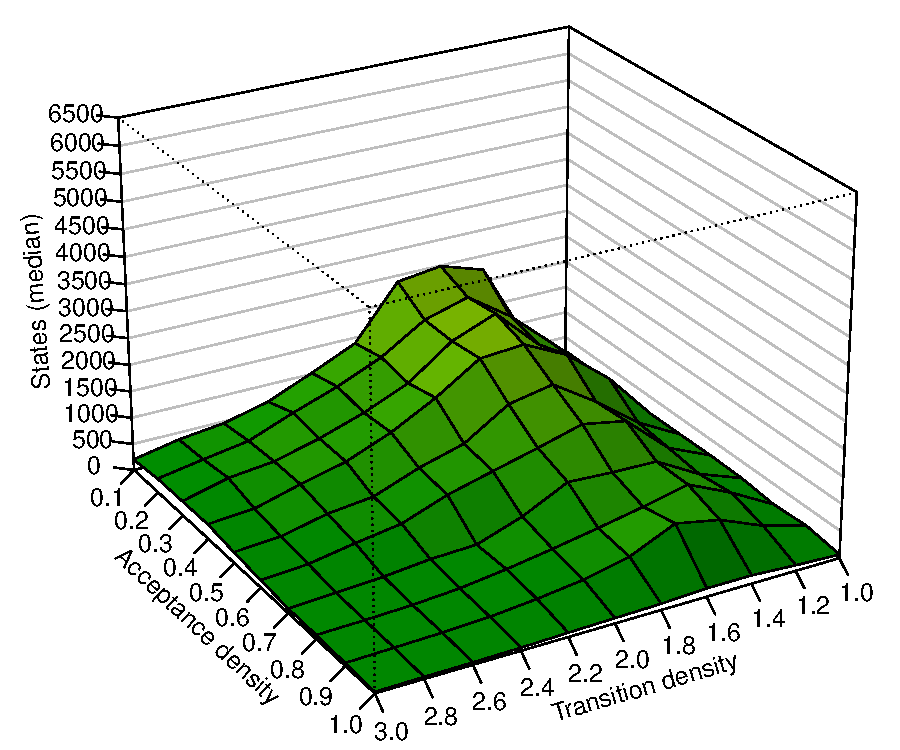
\includegraphics[width=\textwidth]{figures/r/internal/goal/s.median.Fribourg+M1+R2C.pdf}
  \caption{Fribourg+M1+R2C}
  \end{subfigure}
  \hfill

  \hfill
  \begin{subfigure}[t]{\perspwidth\textwidth}
  \centering
  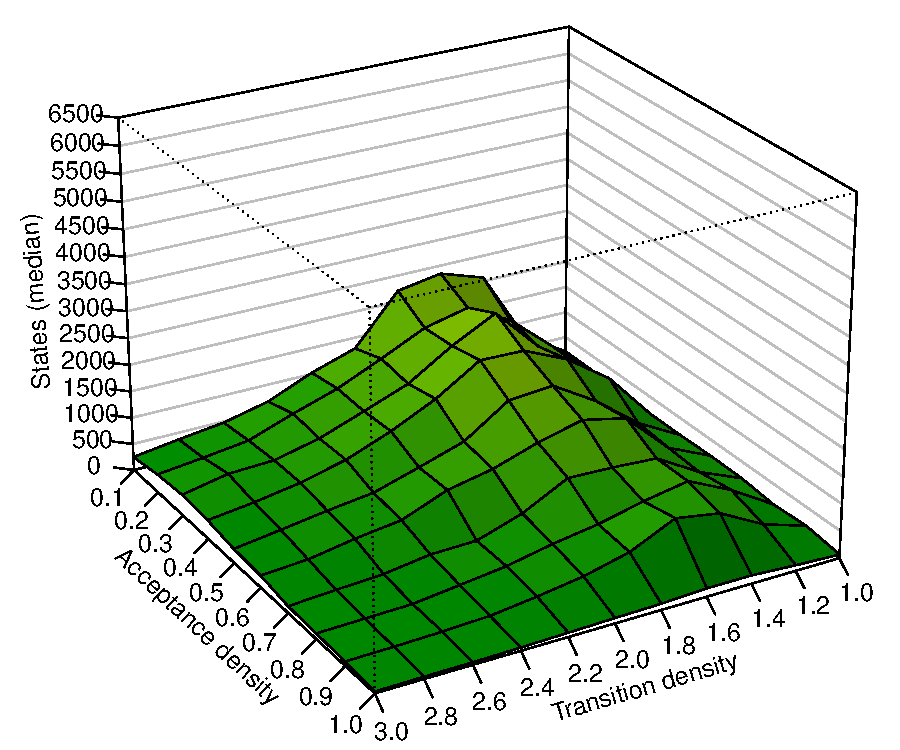
\includegraphics[width=\textwidth]{figures/r/internal/goal/s.median.Fribourg+M1+M2.pdf}
  \caption{Fribourg+M1+M2}
  \end{subfigure}
  \hfill
  \begin{subfigure}[t]{\perspwidth\textwidth}
  \centering
  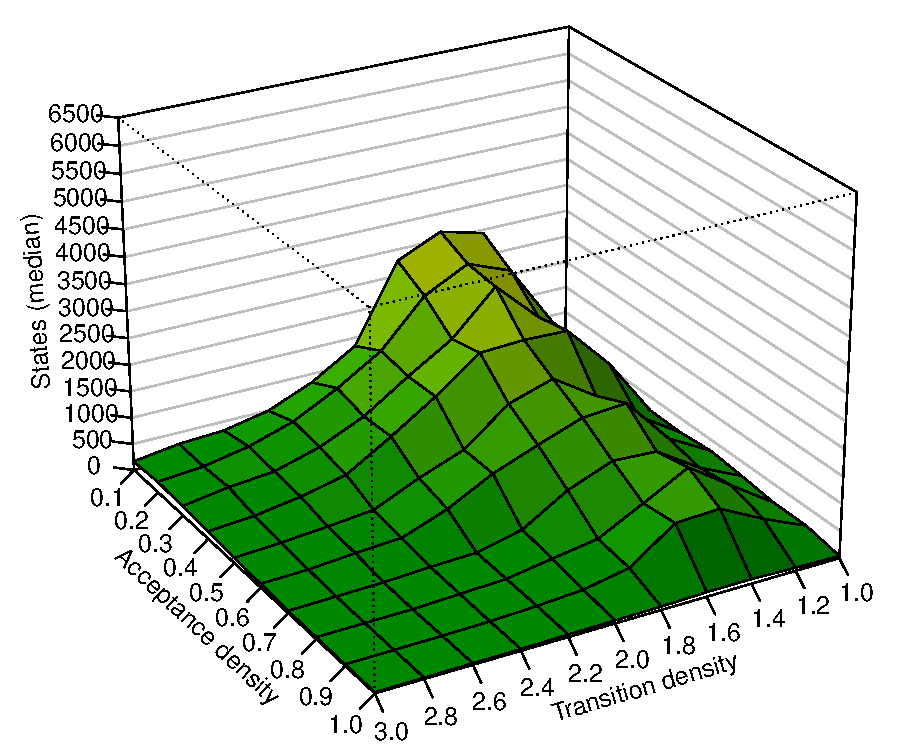
\includegraphics[width=\textwidth]{figures/r/internal/goal/s.median.Fribourg+M1+R2C+C.pdf}
  \caption{Fribourg+M1+R2C+C}
  \end{subfigure}
  \hfill
\caption{Median complement sizes of the 10,939 effective samples from the \goal{} test set for each of the 110 classes.}
\label{i.g.persp_2}
\end{figure}

Figure~\ref{i.g.persp_2} shows the perspective plots of the remaining four versions of the Fribourg construction, all of which include the M1 optimisation. Most apparent in these plots is that the mountain that we described for the plots of Fribourg, Fribourg+R2C, and Fribourg+R2C+C is still there, but it is rather a hill than a mountain. For Fribourg+M1, and Fribourg+M1+R2C, the height of the ridge is around 2,500 states. This is reflected by the overall means of these two versions compared to their counterparts without the M1 optimisation, Fribourg, and Fribourg+R2C. The decrease of the overall mean from Fribourg to Fribourg+M1 is by 52\% (from 2004.6 to 963.2) and from Fribourg+R2C to Fribourg+M1+R2C by 52.1\% (from 1955.9 to 937.7). The decreases of the overall medians are by 36.6\% (from 761 to 482), and 35.1\% (from 689 to 447) for the same two pairs of versions. With this we can confirm that the M1 optimisation brings a significant performance gain for the automata in the \goal{} test set.

Regarding the M2 optimisation, we can see that the mountain ridge in the Fribourg+M1+M2 perspective plot is slightly lower than the one in the Fribourg+M1 perspective plot. The flatland regions, however, seem to not change much. This is reflected by the overall mean of Fribourg+M1+M2 which is slightly lower than in Fribourg+M1 (958.9 opposed to 963.2). The overall median, on the other hand, is higher for Fribourg+M1+M2 than for Fribourg+M1 (496 opposed to 482). An interpretation of this behaviour is that the application of the M2 optimisation results in smaller complements for \textit{some} input automata. \textcolor{red}{Better analysis: Fribourg+M1+M2 is better for almost all classes with an acceptance density up to 0.4, and worse for most of the classes with a n acceptance density between 0.5 and 0.9. The results are exactly identical for all the classes with an acceptance density of 1.0!}. \textcolor{gray}{These automata are especially the hard ones that produce large complements. This positive effect of M2 does however not affect enough input automata, especially not the easy automata, as to improve the overall performance of the construction in terms of the median complement sizes. As already stated previously, we consider therefore Fribourg+M1 as the better construction on the \goal{} test set than Fribourg+M1+M2.}

Finally,Fribourg+M1+R2C+C differs from Fribourg+M1+R2C in a similar way that Fribourg+R2C+C differs from Fribourg+R2C. The higher regions get higher and the lower regions get lower, that is, a performance decline on hard automata, but a performance gain on easy automata. The performance gain on the easy automata is however effective enough to decrease the overall median from 447 to 331, which is minus 26\%.

With 331 states, Fribourg+M1+R2C+C has the lowest median of all the versions (apart from the special case Fribourg+R). However, we still declare Fribourg+M1+R2C as the winner on the \goal{} test set, mainly for two reasons. First, while Fribourg+M1+R2C+C has a lower median, the mean is still higher (1062.6 to 937.7 which is a plus of 13.3\%). This results from the complements of the hard automata, which are larger than with Fribourg+M1+R2C. From a practical point of view, the mean might be relevant, because it relates more directly to the required computing resources than the median. Indeed, the execution per complementation task in CPU time is 25.4\% higher for Fribourg+M1+R2C+C than for Fribourg+M1+R2C (all measured execution time in CPU time are presented in Appendix~\ref{app_times}). The increase in the average execution time per automaton is from 4.44 to 5.57 seconds and in the total execution time from 48,572 seconds ($\approx$ 135 hours) to 60,919 seconds ($\approx$ 169 hours). Fribourg+M1+R2C, on the other hand, has the lowest mean of all versions. The second reason that we choose Fribourg+M1+R2C as the winner and not Fribourg+M1+R2C+C is that the C option is not a real part of the construction. It actually modifies the input automata before the construction starts in order to make them better suited for the construction. Fribourg+M1+R2C, on the other hand, includes only construction-specific options.

\subsubsection{Difficulty Categories}
As we have seen, there are big difference in the complement sizes across the different classes of the \goal{} test set. Furthermore, there is a certain pattern throughout the results of all construction versions, namely the mountain. We attempted to categorise the classes of the \goal{} test set into the three groups ``easy'', ``medium'', and ``hard''. To do so, we first averaged the matrices with the median complement sizes of all the eight versions of the Fribourg construction. In this way, we have a mean median complement size for each class. Then we defined two breakpoints that divide the classes into easy, medium, and hard groups. The breakpoints 500 and 1,600 result in an appropriate groups that seem to capture the reality well. The resulting categorisation is shown in Figure~\ref{i.g.difficulty}.

\begin{figure}[ht]
\centering
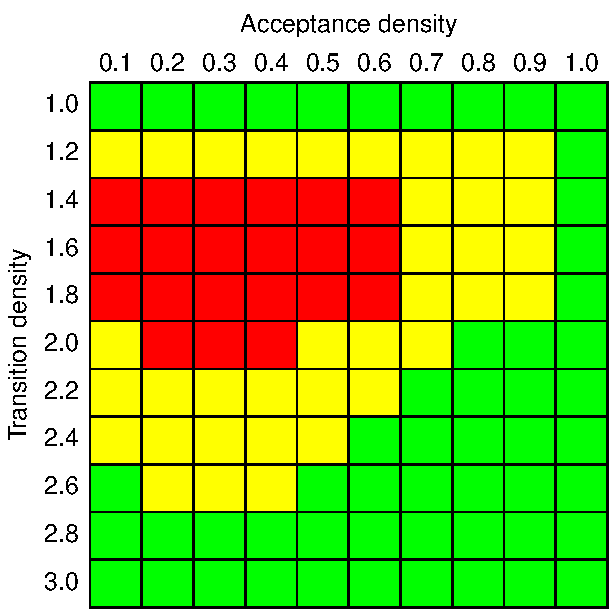
\includegraphics[width=0.35\textwidth]{figures/r/internal/goal/difficulty.pdf}
\caption{Difficulty categories of the 110 \goal{} test set classes. Green: easy; yellow: medium; red: hard.}
\end{figure}

As can be seen in Figure~\ref{i.g.difficulty}, there are 53 easy, 36 medium, and 21 hard classes. The easy classes are mainly those with extreme values. In particular, all the classes with a low or high transition density of 0.1, or 2.8 and 3.0, and a high acceptance density of 1.0 are easy. Furthermore, there is a ``triangle'' of easy classes between transition densities 2.0 and 2.6. and acceptance densities 0.5 and 0.9. The higher the transition density, the lower acceptance density values are tolerated for the class to be easy. The hard classes are roughly those with a transition density between 1.4 and 1.8 and an acceptance density between 0.1 and 0.6. The medium classes finally are grouped as a ``belt'' around the hard classes.

It is interesting that the extreme values of transition density and acceptance density result in easy automata. With a transition density of 1.0 and an alphabet size of 2, each of the 15 states has on average two outgoing and two incoming transitions. With a transition density of 3.0, each state has on average 6 outgoing and 6 incoming transitions. These low or high connectivity seems to considerably simplify the complementation task. The same applies to a high acceptance density of 1.0, which means that every state is an accepting state. Generally, we can say that automata with high acceptance densities are easier to complement than automata with lower acceptance densities. This also means that the pattern of easy automata at the extreme values of transition and acceptance density, does not apply to to the lower extreme of the acceptance density. Automata with a very low acceptance density of 0.1 are hard to complement---unless they are made easy by a low or high transition density.

Another interesting point is that the hard automata have transition densities between 1.4 and 1.8. It seems that this range of transition densities is the crucial factor in the hardness of a complementation task, and that it is only alleviated by a growing acceptance density. This explains the decline of the mountain ridge from low to high acceptance density values.

Summarising we can say that transition densities between 1.4 and 1.8 produce the hardest complementation tasks, and that to the both sides the difficulty steadily decreases with declining or growing transition density. Furthermore, a growing acceptance density generally implies easier complementation tasks.


\subsection{Michel Test Set}
\label{5_internal_michel}
Our second test set consists of the four Michel automata that are listed in Figure~\ref{4_michel_automata} in Section~\ref{4_michel_testset}. They have 3, 4, 5, and 6 states, respectively. The Fribourg construction versions that we tested on the Michel automata are the following.
\begin{enumerate}
\item Fribourg
\item Fribourg+R2C
\item Fribourg+M1
\item Fribourg+M1+M2
\item Fribourg+M1+M2+R2C
\item Fribourg+R
\end{enumerate}

The resulting complement sizes are listed in Table~\ref{i.m.states}.

\begin{table}[htb]
\centering
% latex table generated in R 3.1.2 by xtable 1.7-4 package
% Sun Aug 16 00:19:45 2015
\begin{tabular}{lrrrrrr}
  \hline
Construction & Michel 1 & Michel 2 & Michel 3 & Michel 4 & Fitted curve & Std. error \\ 
  \hline
Fribourg & 57 & 843 & 14,535 & 287,907 & $(1.35n)^n$ & 0.01\% \\ 
  Fribourg+R2C & 33 & 467 & 8,271 & 168,291 & $(1.24n)^n$ & 0.06\% \\ 
  Fribourg+M1 & 44 & 448 & 5,506 & 81,765 & $(1.10n)^n$ & 0.07\% \\ 
  Fribourg+M1+M2 & 42 & 402 & 4,404 & 57,116 & $(1.03n)^n$ & 0.12\% \\ 
  Fribourg+M1+M2+R2C & 28 & 269 & 3,168 & 43,957 & $(0.99n)^n$ & 0.04\% \\ 
  Fribourg+R & 18 & 95 & 528 & 3,315 & $(0.64n)^n$ & 0.35\% \\ 
   \hline
\end{tabular}

\caption{Complement sizes of the Michel automata with $m=\{1,\dots,4\}$ and 3, 4, 5, and 6 states, respectively. }
\label{i.m.states}
\end{table}

In the second-last column ``Fitted curve'' of Table~\ref{i.m.states}, we fitted a function of the form $(an)^n$ to the measured four data points. These data points consist of the sizes of the four Michel automata (3, 4, 5, and 6) as the $x$-values ad the corresponding complement sizes as the $y$-values. The fitted function $(an)^n$ can be seen as an ``averaged'' state growth of these four automata ($n$ is the size of the input automaton). The last column ``Std. error'' contains the standard error that resulted from the fit.

We can see in Table~\ref{i.m.states} that the state growths are indeed very large. For example, complementing Michel~4, which has six states, with the plain Fribourg construction results in a complement of 287,907 states. However, the optimisations R2C, M1, and M2 have a large influence on the complement sizes. If we consider Michel~4, then the R2C optimisation alone reduces the complement size from 287,907 to 168,291 which is a reduction of 51.5\%. The M1 optimisation has an eve larger influence as it reduces the complement size from 287,907 to 81,765 which is a reduction of 71.6\%. Adding M2 to M1 further reduces the complement size of Fribourg+M1 by 30.1\% (from 81,765 to 57,116). Finally, adding R2C on top of M1 and M2 brings a further reduction of of 23\% (from 57,116 to 43,957). If we compare the most efficient version (Fribourg+M1+M2+R2C) with the least efficient one (Fribourg), then the complement size of the former version is only 15.3\% of the complement size of the latter version.

It is interesting to see that for the Michel automata Fribourg+M1+M2 is more efficient than Fribourg+M1. For the \goal{} test set, Friburg+M1+M2 had a slightly higher median than Fribourg+M1 although it had a slightly lower mean. We identified in Section~\ref{5_internal_goal} that the M2 optimisation has a positive effect only on some automata, and that these are mostly the hard automata \textcolor{red}{(The automata with acceptance densities up to 0.4)}. Michel automata are very hard automata \textcolor{red}{(The acceptance densities of the four tested Michel automata are 0.25 or less)}, and indeed the M2 optimisation has a considerably positive effect. These results support thus the observation we made in Section~\ref{5_internal_goal}.

The special version Fribourg+R yields very small complements compared to the other versions. This tells us that the complements of the other versions contain a large number of unreachable and dead states. For example, the complement of Michel~4 of Fribourg+R (3,315 states) is 1.2\% of the size of the complement of Fribourg. This means that 98.8\% of the 287,907 states of the complement of Fribourg are unreachable and dead states. This is actually not surprising, because, following the proof of Michel~\cite{michel1988}\cite{1996_thomas}, the smallest possible complement of Michel~4 has 24 states. This is because Michel~4 has $m=4$ and Michel proved that the complement has at least size $m!$. This means that that even after reducing all the unreachable and dead states from the complement of Fribourg, an even much smaller complement would still be possible.

Up to now we just looked at the specific results of Michel~4. The fitted functions of the form $(an)^n$ summarise the results of all the four Michel automata. These functions give us reference points for the worst-case state complexities of the different versions of the Fribourg construction. For example, for the plain Fribourg construction with its fitted function of $(1.35n)^n$, we have now the proof that this construction produces complements of size $(1.35n)^n$, where $n$ is the size of the input automaton. This means that the worst-case complexity cannot be lower than $(1.35n)^n$ (but it can still be higher). This bound decreases for the different versions of the Fribourg construction down to $(0.99n)^n$ for Fribourg+M1+M2+R2C.

In Table~\ref{i.m.times} we show the measured execution time in seconds (CPU time) for each complementation task. We can see that the difference between the least and most efficient version is bigger than for the complement sizes. For example for Michel~4, Fribourg+M1+M2+R2C is more than 43 times faster than Fribourg (2,332.6 seconds compared to 100,976 seconds). In more familiar unities, this corresponds to approximately 39 minutes for Fribourg+M1+M2+R2C against 28 hours for Fribourg. We also fitted functions of the form $(an)^n$ to the measured execution times where $n$ is the number of states of the input automaton, and the value of the function is the execution time of the task in CPU time seconds.

\begin{table}[htb!]
\centering
% latex table generated in R 3.1.2 by xtable 1.7-4 package
% Sun Aug 16 16:21:25 2015
\begin{tabular}{lrrrrrr}
  \hline
Construction & Michel 1 & Michel 2 & Michel 3 & Michel 4 & Fitted curve & Std. error \\ 
  \hline
Piterman+EQ+RO & 2.5 & 3.8 & 42.6 & 75,917.4 & $(1.08n)^n$ & 0.64\% \\ 
  Slice+P+RO+MADJ+EG & 2.3 & 3.6 & 11.4 & 159.5 & $(0.39n)^n$ & 0.38\% \\ 
  Rank+TR+RO & 2.2 & 3.0 & 6.4 & 30.0 & $(0.29n)^n$ & 0.18\% \\ 
  Fribourg+M1+M2+R2C & 2.5 & 3.5 & 10.8 & 2,332.6 & $(0.61n)^n$ & 0.62\% \\ 
   \hline
\end{tabular}

\caption{Execution time in seconds (CPU time) for complementing the Michel automata~1 to~4.}
\label{i.m.times}
\end{table}

The fitted functions that we calculated for the measured complement sizes and execution times are based on only four data points. This is generally not enough to make reliable extrapolations. However, it is still interesting to do such an extrapolation in order to see the involved complexity and to show why we were restricted to include only the first four Michel automata in the test set. In Table~\ref{i.m.extrapolation}, we show extrapolated values for the complement sizes and execution times for the plain Fribourg construction (the least efficient one), based on the corresponding fitted functions. The table includes the extrapolated values for the Michel automata 5 to 8, which have 7 to 10 states. 


\begin{table}[htb]
\centering
\begin{tabular}{lrrrr}
\hline
Automaton & States ($n$) & Compl. size $(1.35n)^n$ & Exec. time $(1.14n)^n$ & $\approx$ days/months/years \\
\hline
Michel 5 &  7 &       6,882,980 &      2,020,385 &     23 days   \\
Michel 6 &  8 &     189,905,394 &     46,789,245 &     18 months \\
Michel 7 &  9 &   5,939,189,262 &  1,228,250,634 &     39 years  \\
Michel 8 & 10 & 207,621,228,081 & 36,039,825,529 &  1,142 years  \\
\hline
\end{tabular}
\caption{Extrapolated values for the complement sizes and execution times (seconds CPU time)  for the Michel automata with $m=\{5,\dots,10\}$ with the Fribourg version of the Fribourg construction.}
\label{i.m.extrapolation}
\end{table}

According to the fitted state growth function, the complement of Michel~5 would have nearly 7 million states, and the complement of Michel~8 even more than 207 billion states. Already the computation of the 7 million states of Michel~5 would most probably exceed the available memory resources in our computing environment. Regarding execution time, the complementation of Michel~5 would take 23 days. This would by far exceed the maximal running time of a job on our computer cluster. And even if we would not have these administrative time restriction, the time to wait for the complementation of Michel~5 to~8, between 18 months and 1,142 years, is definitely too long, even for a master's thesis.


\section{External Tests}
\label{5_external}
In the external tests we compared the most efficient version of the Fribourg construction to three other constructions. These constructions are Piterman+EQ+RO, Slice+P+RO+MADJ+EG, and Rank+TR+RO. The most efficient version of the Fribourg construction is Fribourg+M1+R2C for the \goal{} test set, and Fribourg+M1+M2+R2C for the Michel test set. We present the results from these two test sets separately in the following two sections.


\subsection{GOAL Test Set}
\label{5_external_goal}
As for the internal tests on the \goal{} test set, we set a time limit of 600 seconds CPU time, and a Java heap size limit of 1 GB per complementation task.  Table~\ref{e.g.outs} shows the number of timeouts and memory excesses that we observed for the four constructions.

\begin{table}[ht]
\centering
% latex table generated in R 3.1.2 by xtable 1.7-4 package
% Sat Jun  6 16:42:17 2015
\begin{tabular}{lrr}
  \hline
Construction & Timeouts & Memory excesses \\ 
  \hline
Fribourg & 48 & 0 \\ 
  Fribourg+R2C & 30 & 0 \\ 
  Fribourg+R2C+C & 54 & 0 \\ 
  Fribourg+M1 & 2 & 0 \\ 
  Fribourg+M1+M2 & 1 & 0 \\ 
  Fribourg+M1+R2C & 1 & 0 \\ 
  Fribourg+M1+R2C+C & 8 & 0 \\ 
  Fribourg+R & 48 & 0 \\ 
   \hline
\end{tabular}

\caption{Number of timeouts and memory excesses for the \goal{} test set.}
\label{e.g.outs}
\end{table}

\subsubsection{With Rank}

Most salient in Table~\ref{e.g.outs} is the high number of aborted tasks for the Rank construction. 3,317 of the 11,000 automata (33.8\%) were aborted due to a timeout, and further 83 (0.8\%) due to a memory excess. Regarding the other constructions, there are just two timeouts for the Piterman construction, and a single timeout for the Fribourg construction.

Determining the effective samples of these runs gives a number of 7,204 automata, which is 65.5\% of the total number of automata. In Figure~\ref{e.g.stripchart.with_rank} we present the complement sizes of these 7,204 effective samples as a stripchart. 

\begin{figure}[ht]
\centering
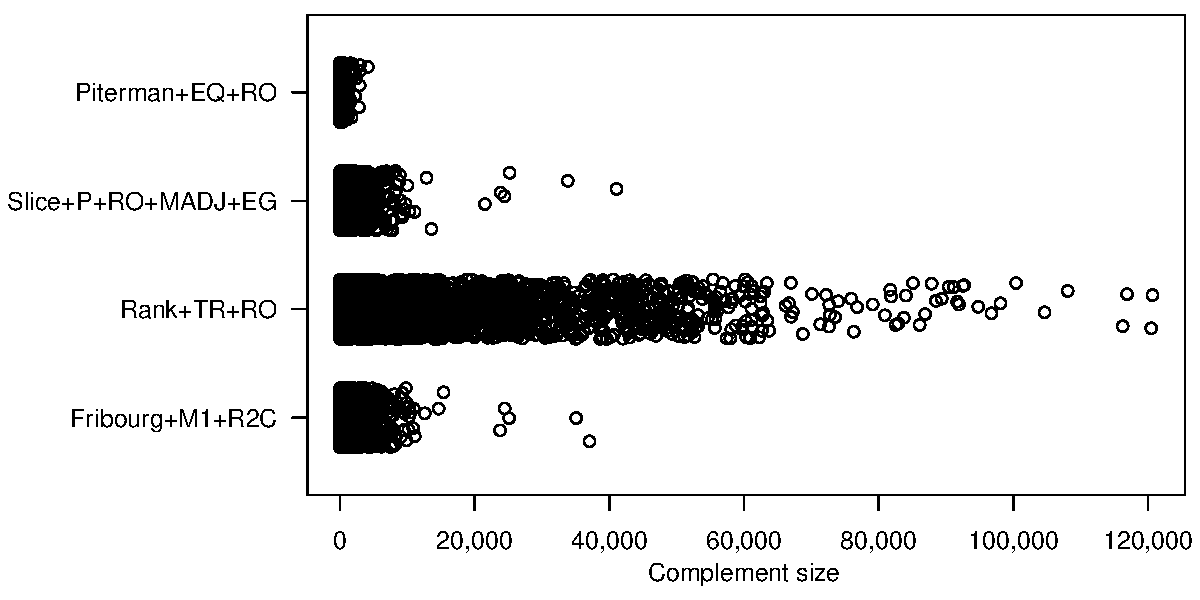
\includegraphics[width=0.75\textwidth]{figures/r/external/goal/s.stripchart.with_rank.pdf}
\caption{Complement sizes of the 7,204 effective samples.}
\label{e.g.stripchart.with_rank}
\end{figure}

The stripchart makes the reason for the high number of aborted tasks of the Rank construction apparent. Rank+TR+RO produces a high number of very large complements compared to the other constructions.

But from the stripchart in Figure~\ref{e.g.stripchart} alone we cannot yet tell whether the Rank construction \textit{generally} produces larger complements than the other constructions, or if this holds just for \textit{some} automata. To this end we have to inspect the statistics about the distribution of the complement sizes in Table~\ref{e.g.stats.with_rank}.

\begin{table}[ht]
\centering
% latex table generated in R 3.1.2 by xtable 1.7-4 package
% Sun Aug 16 15:57:19 2015
\begin{tabular}{lrrrrrr}
  \hline
Construction & Mean & Min. & P25 & Median & P75 & Max. \\ 
  \hline
Piterman+EQ+RO & 106.0 & 1 & 29.0 & 58.0 & 121.0 & 4,126 \\ 
  Slice+P+RO+MADJ+EG & 555.4 & 2 & 70.0 & 202.0 & 596.0 & 41,081 \\ 
  Rank+TR+RO & 5,255.6 & 2 & 81.0 & 254.5 & 3,178.2 & 120,674 \\ 
  Fribourg+M1+R2C & 662.9 & 2 & 101.0 & 269.0 & 754.5 & 37,068 \\ 
   \hline
\end{tabular}

\caption{Statistics of complement sizes of the 7,204 effective samples}
\label{e.g.stats.with_rank}
\end{table}

And indeed, the 25th percentile and the median of Rank are higher than for Piterman and Slice, but still lower than for our Fribourg construction. This means that the Rank construction produces more smaller complements than the Fribourg construction. However, the picture changes dramatically for the 75th percentile where the value of Rank is more than four times higher than the value for Fribourg. Also the mean of Rank is many times higher than the means of all the other constructions. A possible explanation for this is that the Rank construction has a comparable performance with the other constructions for easy automata. For harder automata, however, the performance of Rank is much worse than the other constructions. In addition, the automata that are hardest for Rank are not even included in this analysis as it includes only the 7,204 effective samples. The 3,796 automata that are excluded would probably have resulted in even larger complements with the Rank construction.

What we cannot tell is whether the automata which are hard for Rank are the same that are hard for the other constructions. However, as we will see later, we think that this is not necessarily the case.

\subsubsection{Without Rank}

Given the large number of aborted complementation tasks of Rank we decided to do the main analysis and comparison of the results without the Rank construction. Because with the Rank construction would basically exclude more than one third of the tasks that have been successfully completed by the other constructions from the result analysis. Our main interest is however to compare the performance of the Fribourg construction to the other constructions. In this way, we would probably miss important aspects in the result analysis of the other three constructions. 

Without the Rank construction there are 10,998 effective samples In Figure~\ref{e.g.stripchart} we display the complement sizes of these 10,998 effective samples as a stripchart.

\begin{figure}[ht]
\centering
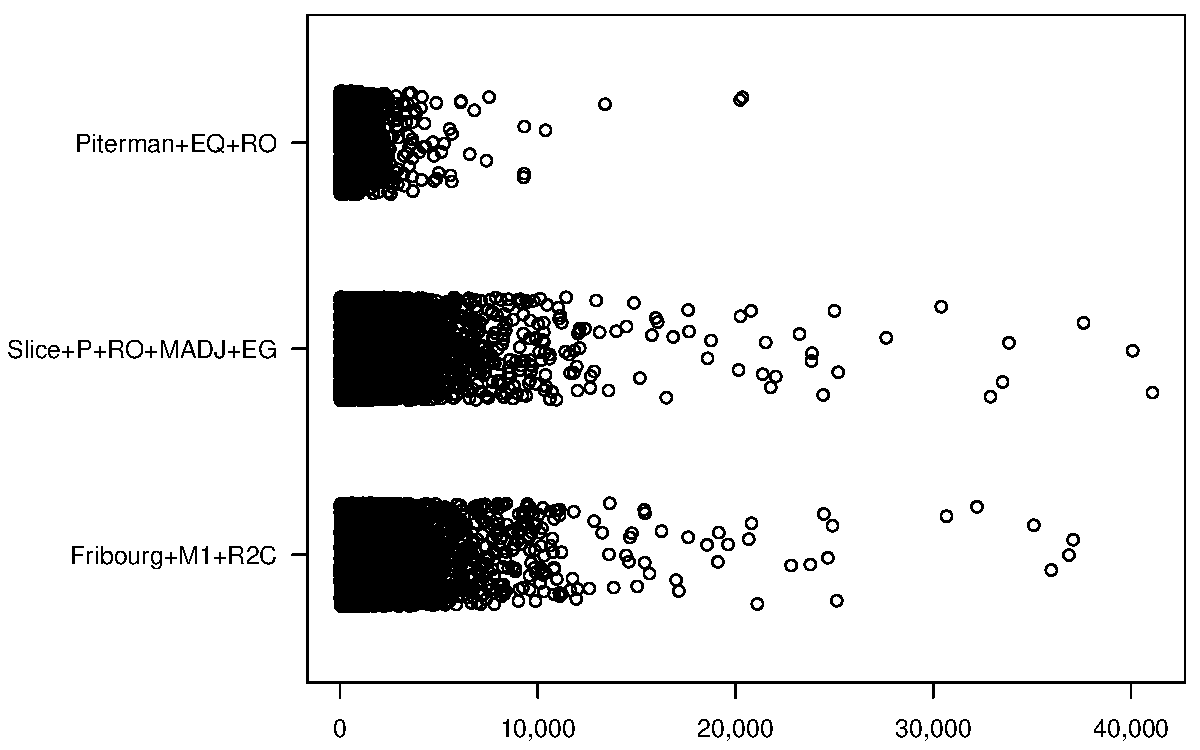
\includegraphics[width=0.75\textwidth]{figures/r/external/goal/s.stripchart.pdf}
\caption{Complement sizes of the 10,998 effective samples.}
\label{e.g.stripchart}
\end{figure}

From the stripchart we can see that Fribourg and Slice have a comparable distribution of complement sizes, whereas Piterman has a considerably higher concentration of small complement sizes. We can say that Piterman generally produces smaller complement than Fribourg and Slice.

We present the statistics of these distributions in Table~\ref{e.g.stats}. 
Indeed, for all statistics Piterman has values that are multiple times lower than the ones of Fribourg and Slice. It is interesting that for mean, 25th percentile, median, and 75th percentile the values of Piterman are more or less five times smaller. It seems like Piterman would produce complements that are throughout five times smaller than the complements of Fribourg and Slice.

\begin{table}[ht]
\centering
% latex table generated in R 3.1.2 by xtable 1.7-4 package
% Sat Jun  6 16:42:20 2015
\begin{tabular}{lrrrrrr}
  \hline
Construction & Mean & Min. & P25 & Median & P75 & Max. \\ 
  \hline
Piterman+EQ+RO & 209.6 & 1 & 38.0 & 80.0 & 183.0 & 20,349 \\ 
  Slice+P+RO+MADJ+EG & 949.4 & 2 & 120.0 & 396.0 & 1,003.0 & 41,081 \\ 
  Fribourg+M1+R2C & 1,017.3 & 2 & 153.0 & 452.0 & 1,134.0 & 37,068 \\ 
   \hline
\end{tabular}

\caption{Aggregated statistics of complement sizes of the 10,998 effective samples without Rank.}
\label{e.g.stats}
\end{table}

Comparing Fribourg and Slice, there is a slight advantage for Slice. Mean, 25th percentile, median, and 75th percentile are lower for Slice than for Fribourg by 6.7\%, 21.6\%, 12.4\%, and 11.6\%, respectively. We have to conclude that from an overall point of view, the Fribourg construction has the second-worst performance for the \goal{} test set after Piterman and Slice, and before Rank.

Figure~\ref{e.g.persp} shows the perspective plots with the median complement sizes for the 110 classes of the 10,998 samples. As already mentioned, the corresponding matrices can be found in Appendix~\ref{app_matrices}.


\renewcommand{\perspwidth}{0.3}
\begin{figure}[ht]
\centering
  \hfill
  \begin{subfigure}[t]{\perspwidth\textwidth}
  \centering
  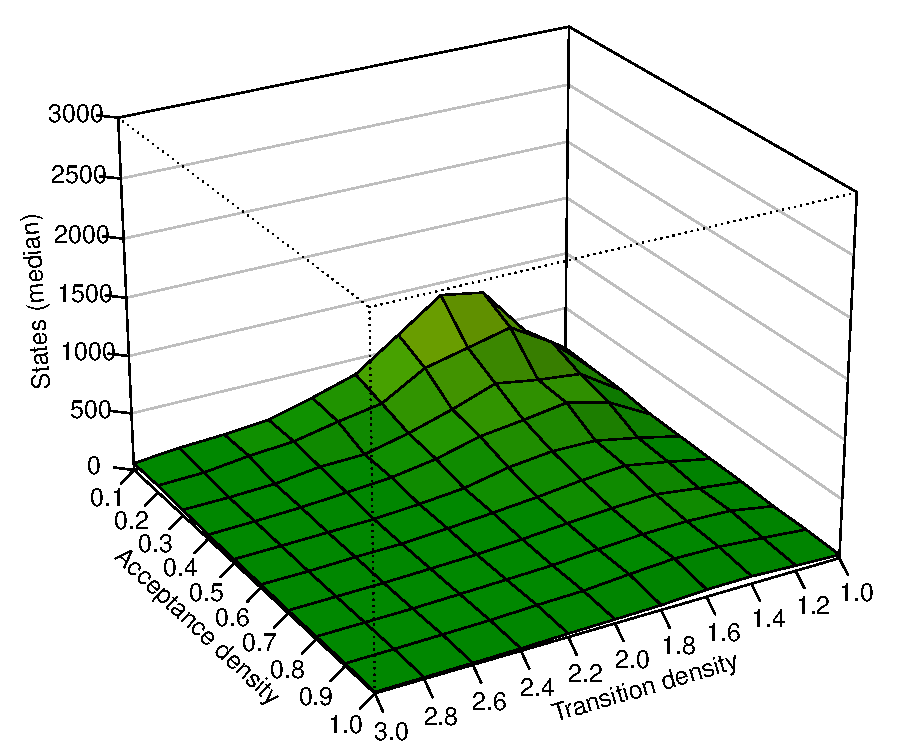
\includegraphics[width=\textwidth]{figures/r/external/goal/s.median.Piterman+EQ+RO.pdf}
  \caption{Piterman+EQ+RO}
  \end{subfigure}
  \hfill
  \begin{subfigure}[t]{\perspwidth\textwidth}
  \centering
  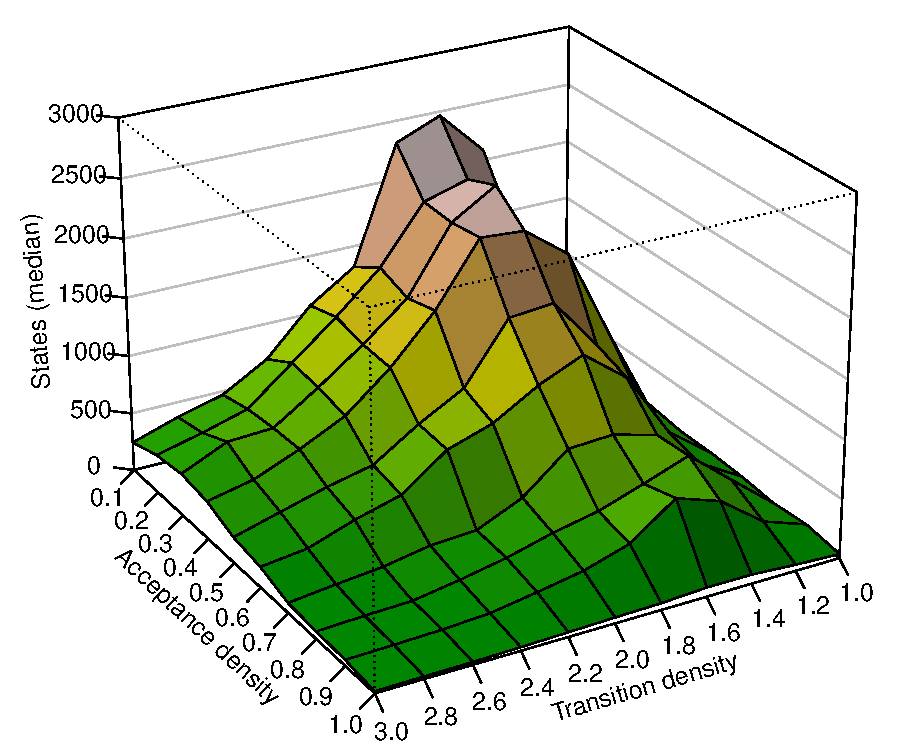
\includegraphics[width=\textwidth]{figures/r/external/goal/s.median.Slice+P+RO+MADJ+EG.pdf}
  \caption{Slice+P+RO+MADJ+EG}
  \end{subfigure}
  \hfill
  \begin{subfigure}[t]{\perspwidth\textwidth}
  \centering
  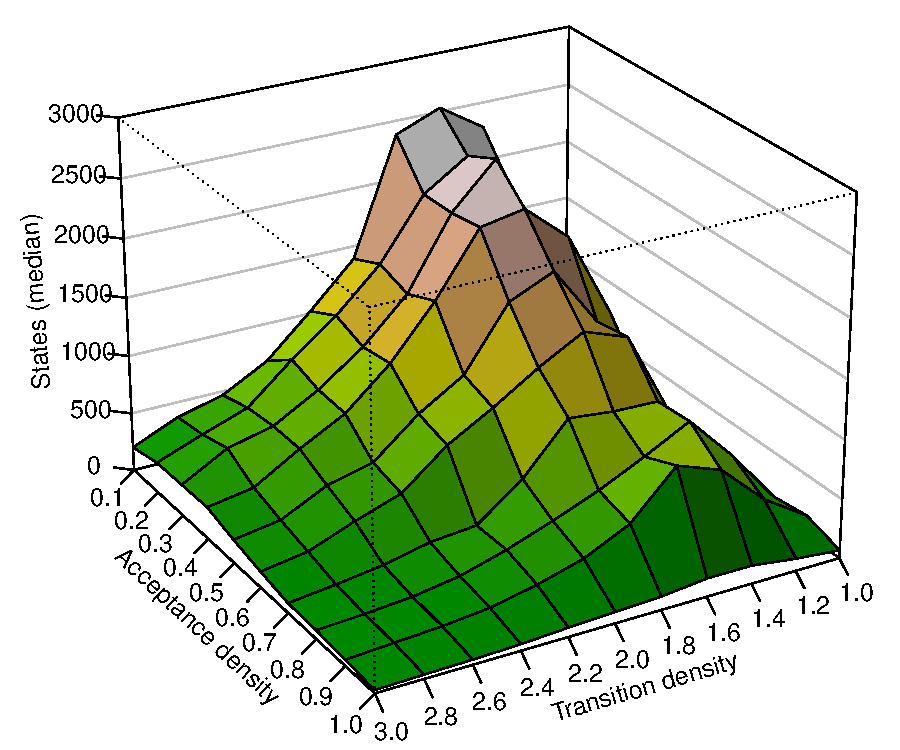
\includegraphics[width=\textwidth]{figures/r/external/goal/s.median.Fribourg+M1+R2C.pdf}
  \caption{Fribourg+M1+R2C}
  \end{subfigure}
  \hfill
\caption{Median complement sizes (10,998 samples)}
\label{e.g.persp}
\end{figure}

Note that the plot of Fribourg+M1+R2C in Figure~\ref{e.g.persp} (c) is the same as the one in Figure~\ref{i.g.persp_2} (b). The only difference is the scale of the vertical axis.

In the perspective plots we can see that the pattern for Fribourg and Slice are very similar. The median complement sizes in the individual classes do not differ a lot, both relatively and absolutely. However, the medians of Fribourg seem to be throughout (with some exceptions) slightly higher than the ones of Slice. This means that Fribourg and Slice seem to have similar strengths and weaknesses, but Slice is slightly more efficient on the tested automata.

Piterman, as expected, has medians that are multiple times lower than the corresponding medians of Fribourg and Slice. The basic pattern, however, is still similar. There is a mountain ridge along the classes with a transition density of 1.6 with its top in the class with transition density 1.6 and acceptance density 0.1.


\subsection{Michel Test Set}
\label{5_external_michel}
For the Michel test set we used the same three third-party construction as for the \goal{} test set, namely Piterman+EQ+RO, Slice+P+RO+MADJ+EG, and Rank+TR+RO. The used Fribourg construction version is however Fribourg+M1+M2+R2C, as this is the most efficient version of the Fribourg construction on the Michel test set.

The resulting complement sizes are shown in Table~\ref{e.m.states}. Again, we fitted a function of the form $(an)^n$ to the four measured data points of each construction and calculated the standard error of this fit.

\begin{figure}[ht]
\centering
% latex table generated in R 3.1.2 by xtable 1.7-4 package
% Sun Aug 16 00:19:45 2015
\begin{tabular}{lrrrrrr}
  \hline
Construction & Michel 1 & Michel 2 & Michel 3 & Michel 4 & Fitted curve & Std. error \\ 
  \hline
Fribourg & 57 & 843 & 14,535 & 287,907 & $(1.35n)^n$ & 0.01\% \\ 
  Fribourg+R2C & 33 & 467 & 8,271 & 168,291 & $(1.24n)^n$ & 0.06\% \\ 
  Fribourg+M1 & 44 & 448 & 5,506 & 81,765 & $(1.10n)^n$ & 0.07\% \\ 
  Fribourg+M1+M2 & 42 & 402 & 4,404 & 57,116 & $(1.03n)^n$ & 0.12\% \\ 
  Fribourg+M1+M2+R2C & 28 & 269 & 3,168 & 43,957 & $(0.99n)^n$ & 0.04\% \\ 
  Fribourg+R & 18 & 95 & 528 & 3,315 & $(0.64n)^n$ & 0.35\% \\ 
   \hline
\end{tabular}

\caption{Complement sizes of the first four Michel automata.}
\label{e.m.states}
\end{figure}

Considering the results of the \goal{} test set, the results in Table~\ref{e.m.states} are surprising. Rank is the most efficient construction. It produces the smallest complements for all Michel automata, and with $(0.91n)^n$ it has the flattest fitted curve of all constructions. This is surprising because for the \goal{} test set, Rank produced by far the largest complements, and 34.5\% of the test data could not even be completed within the given time and memory limits. With the Michel automata, however, the case seems to be reversed and Rank produces by far the smallest complements.

Rank is followed by the Fribourg construction, which has the second-smallest complements for Michel~3 and~4, and with $(0.99n)^n$ the second-flattest fitted curve. The complements of Michel~2, 3, and~4 of the Fribourg construction are bigger than the ones of the Rank construction by 48.6\%, 68.2\%, and 69.2\%, respectively.

The construction with the next steeper fitted curve of $(1.18n)^n$ is the Slice construction. for Michel~1 to~3, this is actually the worst construction, but then for Michel~4, the complement is smaller than the one of Piterman what results in the flatter fitted curve. The gap to the Fribourg construction is big. The complement sizes of Michel~2 to~4 exceed the ones of Fribourg by 60.2\%, 114.2\%, and 180.2\%, respectively. This is also a remarkable point, because for the \goal{} test set, Fribourg and Slice showed a very similar performance.

The last in the ranking is Piterman with a fitted curve of $(1.25n)^n$. However, a special fact for Piterman is that it has the smallest complement for Michel~1 (together with Rank), the second-smallest for Michel~2, the third-smallest for Michel~3, and the largest for Michel~4. It is actually the large complement of Michel~4 that makes Piterman having the steepest fitted curve. However, it is still remarkable that this construction, which is by far the most efficient for the \goal{} test set, produces so much worse results for the Michel automata than all the other constructions. Compared with the Rank construction, Piterman's complements of Michel~2 to~4 are 38.7\%, 174.3\%, and 573.6\%, respectively, bigger. Compared to the Fribourg construction, Piterman produces slightly smaller complements for Michel~1 and~2, but larger ones for Michel~3 and~4. Namely, they are 63.1\% and 298.2\% larger than the corresponding ones of the Fribourg construction.

Summarising we can say that the ranking of the constructions for the Michel test set is exactly the reverse of the ranking for the \goal{} test set. The by far worst construction for the \goal{} test set (Rank) is the best one for the Michel test set, and the by far best construction for the \goal{} test set (Piterman) is the worst one for the Michel test set (at least for Michel~4). For the Fribourg construction this means that it ``advances'' from rank 3 for the \goal{} test set to rank 2 for the Michel test set.

In Table~\ref{e.m.times} we present the execution times per complementation task in CPU time seconds. As for the complement sizes, we fitted a function of the form $(an)^n$ to the measured execution times where $n$ is the size of the input automaton.

\begin{table}[ht]
\centering
% latex table generated in R 3.1.2 by xtable 1.7-4 package
% Sun Aug 16 16:21:25 2015
\begin{tabular}{lrrrrrr}
  \hline
Construction & Michel 1 & Michel 2 & Michel 3 & Michel 4 & Fitted curve & Std. error \\ 
  \hline
Piterman+EQ+RO & 2.5 & 3.8 & 42.6 & 75,917.4 & $(1.08n)^n$ & 0.64\% \\ 
  Slice+P+RO+MADJ+EG & 2.3 & 3.6 & 11.4 & 159.5 & $(0.39n)^n$ & 0.38\% \\ 
  Rank+TR+RO & 2.2 & 3.0 & 6.4 & 30.0 & $(0.29n)^n$ & 0.18\% \\ 
  Fribourg+M1+M2+R2C & 2.5 & 3.5 & 10.8 & 2,332.6 & $(0.61n)^n$ & 0.62\% \\ 
   \hline
\end{tabular}

\caption{Execution times for the first four Michel automata.}
\label{e.m.times}
\end{table}

Most interesting in Table~\ref{e.m.times} is the column with the times for Michel~4. The time difference between the best and the worst construction is enormous. While the Rank construction took just 30 seconds to complement Michel~4, the Piterman construction took 75,917.4 seconds which is approximately 21 hours. This is more than 2500 times longer. Of course the Piterman construction produced a bigger automata, which naturally requires more time, however, the automaton produced by the Piterman construction is just around 6.7 times bigger than the one of the Rank construction. This means that the Piterman construction must include very inefficient processes before finally arriving at the output automaton.

Furthermore, we can see in Table~\ref{e.m.times} that also the Fribourg construction took relatively long to complement Michel~4 compared to Rank, namely 2,332.6 seconds which are approximately 39 minutes. This is 77.8 times longer than the 30 seconds of Rank. At the same time, Fribourg's complement has just 68.2\% more states than Rank's complement. Similarly, compared to the Slice construction the Fribourg construction is slow for Michel~4. Slice's complement is 2.8 times bigger than Fribourg's complement, but with 159.5 seconds the complementation of slice was 14.6 times faster than the complementation of Fribourg.

So there seems to an inefficiency in the Fribourg construction in terms of execution time for the complementation of Michel~4. However, this inefficiency is by far not as pronounced as for Piterman. While the complement of Piterman is just 4 times bigger, the execution time of Piterman is 32.5 times longer than the one of the Fribourg construction. One could also look at it from the other side and say that not the Fribourg construction is inefficient on Michel~4, but that Rank and Slice are extremely efficient on this automaton.

Finally, these interesting differences in the execution times between the four constructions can only be observed for Michel~4. For Michel~3 there are also differences but they are by far not as pronounced as for Michel~4. If the computational resources would allow it, it would be very interesting to run the constructions on Michel~5 and beyond. One thing that stays the same for all the four Michel automata is that Rank is always the fastest and Piterman always the slowest construction.

\section{Summary and Discussion of the Results}
\label{5_discussion}

\section{Limitations of the Approach}
\label{5_limitations}
